% This file was created with tikzplotlib v0.10.1.
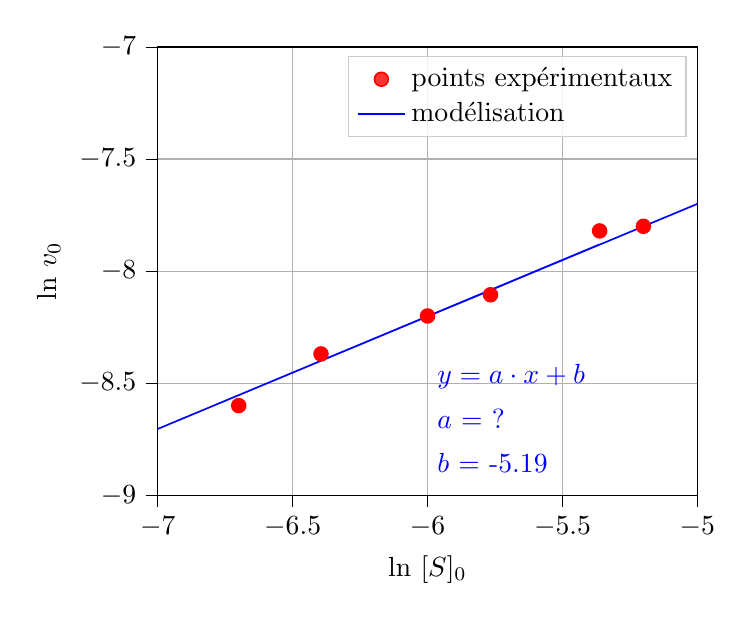
\begin{tikzpicture}

\definecolor{darkgray176}{RGB}{176,176,176}
\definecolor{lightgray204}{RGB}{204,204,204}

\begin{axis}[
legend cell align={left},
legend style={fill opacity=0.8, draw opacity=1, text opacity=1, draw=lightgray204},
tick align=outside,
tick pos=left,
x grid style={darkgray176},
xlabel={ln \(\displaystyle [S]_0\)},
xmajorgrids,
xmin=-7, xmax=-5,
xtick style={color=black},
y grid style={darkgray176},
ylabel={ln \(\displaystyle v_0\)},
ymajorgrids,
ymin=-9, ymax=-7,
ytick style={color=black}
]
\addplot [semithick, red, mark=*, mark size=2.5, mark options={solid}, only marks]
table {%
%-6.394931652553473 -8.399410155759854
-6.394931652553473 -8.369410155759854
%-5.766722274430075 -8.0854107749907
-5.766722274430075 -8.1054107749907
%-5.3623226965239486 -7.8806163623446865
-5.3623226965239486 -7.8206163623446865
-6.7 -8.6
-6 -8.2
-5.2 -7.8
};
\addlegendentry{points expérimentaux}
\addplot [semithick, blue]
table {%
-6.394931652553473 -8.399410155759854
-5.766722274430075 -8.0854107749907
-5.3623226965239486 -7.8806163623446865
-7 -8.704
-5 -7.7
};
\addlegendentry{modélisation}
\draw (axis cs:-6,-8.5) node[
  scale=1,
  anchor=base west,
  text=blue,
  rotate=0.0
]{$y=a\cdot x+b$};
\draw (axis cs:-6,-8.7) node[
  scale=1,
  anchor=base west,
  text=blue,
  rotate=0.0
]{$a$ = ?};
%0.502};
\draw (axis cs:-6,-8.9) node[
  scale=1,
  anchor=base west,
  text=blue,
  rotate=0.0
]{$b$ = \num{-5.19}};
\end{axis}

\end{tikzpicture}
